% TODO: add `final` to hide todonotes
%\documentclass[11pt,a4paper,oneside]{report}             % Single-side
\documentclass[11pt,a4paper,twoside,openright,final]{report}  % Duplex

% thanks to http://tex.stackexchange.com/a/47579/71109
\usepackage{ifxetex}
\usepackage{ifluatex}
\newif\ifxetexorluatex % a new conditional starts as false
\ifnum 0\ifxetex 1\fi\ifluatex 1\fi>0
   \xetexorluatextrue
\fi

\ifxetexorluatex
  \usepackage{fontspec}
\else
  \usepackage[T1]{fontenc}
  \usepackage[utf8]{inputenc}
  \usepackage[lighttt]{lmodern}
  \ttfamily\DeclareFontShape{T1}{lmtt}{m}{it}{<->sub*lmtt/m/sl}{}
\fi

\usepackage[english,magyar]{babel} % Alapértelmezés szerint utoljára definiált nyelv lesz aktív, de később külön beállítjuk az aktív nyelvet.

\usepackage{emptypage} % omit page number on empty pages

%\usepackage{cmap}
\usepackage{amsfonts,amsmath,amssymb} % Mathematical symbols.
%\usepackage[ruled,boxed,resetcount,linesnumbered]{algorithm2e} % For pseudocodes. % beware: this is not compatible with LuaLaTeX, see http://tex.stackexchange.com/questions/34814/lualatex-and-algorithm2e
\usepackage{booktabs} % For publication quality tables for LaTeX
\usepackage{graphicx}

%\usepackage{fancyhdr}
%\usepackage{lastpage}

\usepackage{geometry}
%\usepackage{sectsty}
\usepackage{setspace} % For setting line spacing

\usepackage[unicode]{hyperref} % For hyperlinks in the generated document.
\usepackage{xcolor}
\usepackage{listings} % For source code snippets.

\usepackage[amsmath,thmmarks]{ntheorem} % Theorem-like environments.

\usepackage[hang]{caption}

\singlespacing

\newcommand{\selecthungarian}{
	\selectlanguage{magyar}
	\setlength{\parindent}{2em}
	\setlength{\parskip}{0em}
	\frenchspacing
}

\newcommand{\selectenglish}{
	\selectlanguage{english}
	\setlength{\parindent}{0em}
	\setlength{\parskip}{0.5em}
	\nonfrenchspacing
	\renewcommand{\figureautorefname}{Figure}
	\renewcommand{\tableautorefname}{Table}
	\renewcommand{\partautorefname}{Part}
	\renewcommand{\chapterautorefname}{Chapter}
	\renewcommand{\sectionautorefname}{Section}
	\renewcommand{\subsectionautorefname}{Section}
	\renewcommand{\subsubsectionautorefname}{Section}
}

\usepackage[numbers]{natbib}
\usepackage{xspace}

\usepackage[obeyFinal]{todonotes}
\definecolor{lightblue}{rgb}{0.68, 0.85, 0.9}
\newcommand{\marci}[1]{\todo[color=lightblue]{\textbf{M:} #1}}
\newcommand{\marciLine}[1]{\todo[inline,color=lightblue]{#1}}

\usepackage{forest}
\usepackage{subfiles}


\newcommand{\vikszerzoVezeteknev}{Tieger}
\newcommand{\vikszerzoKeresztnev}{Balázs}

\newcommand{\vikkonzulensAMegszolitas}{}
\newcommand{\vikkonzulensAVezeteknev}{Elekes}
\newcommand{\vikkonzulensAKeresztnev}{Márton}

\newcommand{\vikkonzulensBMegszolitas}{}
\newcommand{\vikkonzulensBVezeteknev}{Szatmári}
\newcommand{\vikkonzulensBKeresztnev}{Zoltán}

\newcommand{\vikkonzulensCMegszolitas}{}
\newcommand{\vikkonzulensCVezeteknev}{}
\newcommand{\vikkonzulensCKeresztnev}{}

\newcommand{\vikcim}{Enforcing Kubernetes constraints using high level Dsl} % Cím
\newcommand{\viktanszek}{\bmemit} % Tanszék
\newcommand{\vikdoktipus}{\msc} % Dokumentum típusa (\bsc vagy \msc)
\newcommand{\vikmunkatipusat}{diplomatervet} % a "hallgató nyilatkozat" részhez: szakdolgozatot vagy diplomatervet


\newcommand{\szerzoMeta}{\vikszerzoVezeteknev{} \vikszerzoKeresztnev} % egy szerző esetén
%\newcommand{\szerzoMeta}{\vikszerzoVezeteknev{} \vikszerzoKeresztnev, \tdkszerzoB} % két szerző esetén


% Beállítások magyar nyelvű dolgozathoz
%%--------------------------------------------------------------------------------------
% Elnevezések
%--------------------------------------------------------------------------------------
\newcommand{\bme}{Budapesti Műszaki és Gazdaságtudományi Egyetem}
\newcommand{\vik}{Villamosmérnöki és Informatikai Kar}

\newcommand{\bmemit}{Méréstechnika és Információs Rendszerek Tanszék}

\newcommand{\keszitette}{Készítette}
\newcommand{\konzulens}{Konzulens}

\newcommand{\bsc}{Szakdolgozat}
\newcommand{\msc}{Diplomaterv}
\newcommand{\tdk}{TDK dolgozat}
\newcommand{\bsconlab}{BSc Önálló laboratórium}
\newcommand{\msconlabi}{MSc Önálló laboratórium 1.}
\newcommand{\msconlabii}{MSc Önálló laboratórium 2.}

\newcommand{\pelda}{Példa}
\newcommand{\definicio}{Definíció}
\newcommand{\tetel}{Tétel}

\newcommand{\bevezetes}{Bevezetés}
\newcommand{\koszonetnyilvanitas}{Köszönetnyilvánítás}
\newcommand{\fuggelek}{Függelék}

% Opcionálisan átnevezhető címek
%\addto\captionsmagyar{%
%\renewcommand{\listfigurename}{Saját ábrajegyzék cím}
%\renewcommand{\listtablename}{Saját táblázatjegyzék cím}
%\renewcommand{\bibname}{Saját irodalomjegyzék név}
%}

\newcommand{\szerzo}{\vikszerzoVezeteknev{} \vikszerzoKeresztnev}
\newcommand{\vikkonzulensA}{\vikkonzulensAMegszolitas\vikkonzulensAVezeteknev{} \vikkonzulensAKeresztnev}
\newcommand{\vikkonzulensB}{\vikkonzulensBMegszolitas\vikkonzulensBVezeteknev{} \vikkonzulensBKeresztnev}
\newcommand{\vikkonzulensC}{\vikkonzulensCMegszolitas\vikkonzulensCVezeteknev{} \vikkonzulensCKeresztnev}

\newcommand{\selectthesislanguage}{\selecthungarian}

\bibliographystyle{huplain}

\def\lstlistingname{kódrészlet}

\newcommand{\appendixnumber}{6}  % a fofejezet-szamlalo az angol ABC 6. betuje (F) lesz

%--------------------------------------------------------------------------------------
% Elnevezések
%--------------------------------------------------------------------------------------
\newcommand{\bme}{Budapest University of Technology and Economics}
\newcommand{\vik}{Faculty of Electrical Engineering and Informatics}

\newcommand{\bmemit}{Department of Measurement and Information Systems}

\newcommand{\keszitette}{Author}
\newcommand{\konzulens}{Advisor}

\newcommand{\bsc}{Bachelor's Thesis}
\newcommand{\msc}{Master's Thesis}
\newcommand{\tdk}{Scientific Students' Association Report}
\newcommand{\bsconlab}{BSc Project Laboratory}
\newcommand{\msconlabi}{MSc Project Laboratory 1}
\newcommand{\msconlabii}{MSc Project Laboratory 2}

\newcommand{\pelda}{Example}
\newcommand{\definicio}{Definition}
\newcommand{\tetel}{Theorem}

\newcommand{\bevezetes}{Introduction}
\newcommand{\koszonetnyilvanitas}{Acknowledgements}
\newcommand{\fuggelek}{Appendix}

% Optional custom titles
%\addto\captionsenglish{%
%\renewcommand*{\listfigurename}{Your list of figures title}
%\renewcommand*{\listtablename}{Your list of tables title}
%\renewcommand*{\bibname}{Your bibliography title}
%}

\newcommand{\szerzo}{\vikszerzoKeresztnev{} \vikszerzoVezeteknev}
\newcommand{\vikkonzulensA}{\vikkonzulensAMegszolitas\vikkonzulensAKeresztnev{} \vikkonzulensAVezeteknev}
\newcommand{\vikkonzulensB}{\vikkonzulensBMegszolitas\vikkonzulensBKeresztnev{} \vikkonzulensBVezeteknev}
\newcommand{\vikkonzulensC}{\vikkonzulensCMegszolitas\vikkonzulensCKeresztnev{} \vikkonzulensCVezeteknev}

\newcommand{\selectthesislanguage}{\selectenglish}

\bibliographystyle{plainnat}

\newcommand{\ie}{i.e.\@\xspace}
\newcommand{\Ie}{I.e.\@\xspace}
\newcommand{\eg}{e.g.\@\xspace}
\newcommand{\Eg}{E.g.\@\xspace}
\newcommand{\etal}{et al.\@\xspace}
\newcommand{\etc}{etc.\@\xspace}
\newcommand{\vs}{vs.\@\xspace}
\newcommand{\viz}{viz.\@\xspace} % videlicet
\newcommand{\cf}{cf.\@\xspace} % confer
\newcommand{\Cf}{Cf.\@\xspace}
\newcommand{\wrt}{w.r.t.\@\xspace} % with respect to
\newcommand{\approximately}{approx.\@\xspace}

\newcommand{\appendixnumber}{1}  % a fofejezet-szamlalo az angol ABC 1. betuje (A) lesz


%--------------------------------------------------------------------------------------
% Page layout setup
%--------------------------------------------------------------------------------------
% we need to redefine the pagestyle plain
% another possibility is to use the body of this command without \fancypagestyle
% and use \pagestyle{fancy} but in that case the special pages
% (like the ToC, the References, and the Chapter pages)remain in plane style

\pagestyle{plain}
\geometry{inner=35mm, outer=25mm, top=28mm, bottom=25mm}

\setcounter{tocdepth}{3}
%\sectionfont{\large\upshape\bfseries}
\setcounter{secnumdepth}{3}

\sloppy % Margón túllógó sorok tiltása.
\widowpenalty=10000 \clubpenalty=10000 %A fattyú- és árvasorok elkerülése
\def\hyph{-\penalty0\hskip0pt\relax} % Kötőjeles szavak elválasztásának engedélyezése


%--------------------------------------------------------------------------------------
% Setup hyperref package
%--------------------------------------------------------------------------------------
\hypersetup{
    % bookmarks=true,            % show bookmarks bar?
    unicode=true,              % non-Latin characters in Acrobat's bookmarks
    pdftitle={\vikcim},        % title
    pdfauthor={\szerzoMeta},    % author
    pdfsubject={\vikdoktipus}, % subject of the document
    pdfcreator={\szerzoMeta},   % creator of the document
    pdfproducer={},    % producer of the document
    pdfkeywords={},    % list of keywords (separate then by comma)
    pdfnewwindow=true,         % links in new window
    colorlinks=true,           % false: boxed links; true: colored links
    linkcolor=black,           % color of internal links
    citecolor=black,           % color of links to bibliography
    filecolor=black,           % color of file links
    urlcolor=black             % color of external links
}


% https://www.overleaf.com/learn/latex/Code_listing

\definecolor{commentsColor}{rgb}{0.1, 0.7, 0.1}
\definecolor{numberingcolor}{rgb}{0.497495, 0.497587, 0.497464}
\definecolor{keywordsColor}{rgb}{0.000000, 0.000000, 0.635294}
\definecolor{stringColor}{rgb}{0.6, 0.05, 0.15}

% \usepackage{fontspec}
% \newfontfamily{\ttconsolas}{Consolas}[Scale=0.8]
\lstset{ %
  backgroundcolor=\color{white},   % choose the background color; you must add \usepackage{color} or \usepackage{xcolor}
  %basicstyle=\ttfamily,        % the size of the fonts that are used for the code
  basicstyle=\ttfamily\footnotesize,
  breakatwhitespace=false,         % sets if automatic breaks should only happen at whitespace
  breaklines=true,                 % sets automatic line breaking
  captionpos=b,                    % sets the caption-position to bottom
  commentstyle=\color{commentsColor}\textit,    % comment style
  deletekeywords={...},            % if you want to delete keywords from the given language
  escapeinside={\%*}{*)},          % if you want to add LaTeX within your code
  extendedchars=true,              % lets you use non-ASCII characters; for 8-bits encodings only, does not work with UTF-8
  frame=tb,	                   	   % adds a frame around the code
  keepspaces=true,                 % keeps spaces in text, useful for keeping indentation of code (possibly needs columns=flexible)
  keywordstyle=\color{keywordsColor}\bfseries,       % keyword style
  language=Java,                   % the language of the code (can be overrided per snippet)
  numbers=left,                    % where to put the line-numbers; possible values are (none, left, right)
  numbersep=5pt,                   % how far the line-numbers are from the code
  numberstyle=\tiny\color{numberingcolor}, % the style that is used for the line-numbers
  rulecolor=\color{black},         % if not set, the frame-color may be changed on line-breaks within not-black text (e.g. comments (green here))
  showspaces=false,                % show spaces everywhere adding particular underscores; it overrides 'showstringspaces'
  showstringspaces=false,          % underline spaces within strings only
  showtabs=false,                  % show tabs within strings adding particular underscores
  stepnumber=1,                    % the step between two line-numbers. If it's 1, each line will be numbered
  stringstyle=\color{stringColor}, % string literal style
  tabsize=2,	                   % sets default tabsize to 2 spaces
  title=\lstname,                  % show the filename of files included with \lstinputlisting; also try caption instead of title
  columns=fixed                    % Using fixed column width (for e.g. nice alignment)
}



\lstdefinelanguage{Java11}{
  morekeywords={var, void, public, private, new, final, class, protected, abstract, static, import, package, return, boolean, synchronized, if, else, throws, int, throw, null, try, catch, for, while},
  sensitive=true, % keywords are not case-sensitive
  morecomment=[l]{//}, % l is for line comment
  morecomment=[s]{/*}{*/}, % s is for start and end delimiter
  morestring=[b]" % defines that strings are enclosed in double quotes
}

\lstdefinelanguage{MySQL}{
  morekeywords={INSERT, IGNORE, INTO, VALUES},
  sensitive=true, % keywords are not case-sensitive
  morestring=[b]' % defines that strings are enclosed in double quotes
}

\lstdefinelanguage{Kotlin}{
  morekeywords={fun, class, object, var, val, if, else, internal, return, private, by, data, annotation, typealias, infix},
  sensitive=true, % keywords are not case-sensitive
  morecomment=[l]{//}, % l is for line comment
  morecomment=[s]{/*}{*/}, % s is for start and end delimiter
  morestring=[b]" % defines that strings are enclosed in double quotes
}

\lstdefinelanguage{JSON}{
  morekeywords={null, true, false},
  sensitive=true, % keywords are not case-sensitive
  morecomment=[l]{//}, % l is for line comment
  morecomment=[s]{/*}{*/}, % s is for start and end delimiter
  morestring=[b]" % defines that strings are enclosed in double quotes
}

\lstdefinelanguage{YAML}{
  morekeywords={null, true, false},
  sensitive=true, % keywords are not case-sensitive
  morecomment=[l]{\#}, % l is for line comment
  morestring=[b]" % defines that strings are enclosed in double quotes
}

%--------------------------------------------------------------------------------------
% Set up theorem-like environments
%--------------------------------------------------------------------------------------
% Using ntheorem package -- see http://www.math.washington.edu/tex-archive/macros/latex/contrib/ntheorem/ntheorem.pdf

\theoremstyle{plain}
\theoremseparator{.}
\newtheorem{example}{\pelda}

\theoremseparator{.}
%\theoremprework{\bigskip\hrule\medskip}
%\theorempostwork{\hrule\bigskip}
\theorembodyfont{\upshape}
\theoremsymbol{{\large \ensuremath{\centerdot}}}
\newtheorem{definition}{\definicio}

\theoremseparator{.}
%\theoremprework{\bigskip\hrule\medskip}
%\theorempostwork{\hrule\bigskip}
\newtheorem{theorem}{\tetel}


%--------------------------------------------------------------------------------------
% Some new commands and declarations
%--------------------------------------------------------------------------------------
\newcommand{\code}[1]{{\upshape\ttfamily\scriptsize\indent #1}}
\newcommand{\doi}[1]{DOI: \href{http://dx.doi.org/\detokenize{#1}}{\raggedright{\texttt{\detokenize{#1}}}}} % A hivatkozások közt így könnyebb DOI-t megadni.

\DeclareMathOperator*{\argmax}{arg\,max}
%\DeclareMathOperator*[1]{\floor}{arg\,max}
\DeclareMathOperator{\sign}{sgn}
\DeclareMathOperator{\rot}{rot}


%--------------------------------------------------------------------------------------
% Setup captions
%--------------------------------------------------------------------------------------
\captionsetup[figure]{aboveskip=10pt}

\renewcommand{\captionlabelfont}{\bf}
%\renewcommand{\captionfont}{\footnotesize\it}

%--------------------------------------------------------------------------------------
% Hyphenation exceptions
%--------------------------------------------------------------------------------------
\hyphenation{Shakes-peare Mar-seilles ár-víz-tű-rő tü-kör-fú-ró-gép}


\author{\vikszerzo}
\title{\viktitle}


%--------------------------------------------------------------------------------------
% Table of contents and the main text
%--------------------------------------------------------------------------------------
\begin{document}

\pagenumbering{gobble}


\selectthesislanguage


%~~~~~~~~~~~~~~~~~~~~~~~~~~~~~~~~~~~~~~~~~~~~~~~~~~~~~~~~~~~~~~~~~~~~~~~~~~~~~~~~~~~~~~
\hypersetup{pageanchor=false}
%--------------------------------------------------------------------------------------
%	The title page
%--------------------------------------------------------------------------------------
\begin{titlepage}
\begin{center}

\includegraphics[width=60mm,keepaspectratio]{figures/bme_logo.pdf}\\
\vspace{0.3cm}
\textbf{\bme}\\
\textmd{\vik}\\
\textmd{\viktanszek}\\[5cm]

\vspace{0.4cm}
{\huge \bfseries \vikcim}\\[0.8cm]
\vspace{0.5cm}
\textsc{\Large \vikdoktipus}\\[4cm]

{
	\renewcommand{\arraystretch}{0.85}
	\begin{tabular}{cc}
	 \makebox[7cm]{\emph{\keszitette}} & \makebox[7cm]{\emph{\konzulens}} \\ \noalign{\smallskip}
	 \makebox[7cm]{\szerzo} & \makebox[7cm]{\vikkonzulensA} \\
	  & \makebox[7cm]{\vikkonzulensB} \\
	  & \makebox[7cm]{\vikkonzulensC} \\
	\end{tabular}
}

%\todo[inline]{Add final to \textbackslash documentclass in thesis.tex to hide todos; check that there are no remaining todos (and \textbackslash listoftodos) by commenting \textbackslash usepackage ... todonotes out in packages.tex}

\vfill
{\large \today}
\end{center}
\end{titlepage}
\hypersetup{pageanchor=false}

		   % Szakdolgozat/Diplomaterv címlap

%\listoftodos

% Table of Contents
%~~~~~~~~~~~~~~~~~~~~~~~~~~~~~~~~~~~~~~~~~~~~~~~~~~~~~~~~~~~~~~~~~~~~~~~~~~~~~~~~~~~~~~
\setcounter{tocdepth}{1}
\tableofcontents\cleardoublepage


% Declaration and Abstract
%~~~~~~~~~~~~~~~~~~~~~~~~~~~~~~~~~~~~~~~~~~~~~~~~~~~~~~~~~~~~~~~~~~~~~~~~~~~~~~~~~~~~~~
% \selectlanguage{magyar}
\pagenumbering{gobble}
%--------------------------------------------------------------------------------------
% Nyilatkozat
%--------------------------------------------------------------------------------------
\begin{center}
\large
\textbf{HALLGATÓI NYILATKOZAT}\\
\end{center}

Alulírott \emph{\vikszerzoVezeteknev{} \vikszerzoKeresztnev}, szigorló hallgató kijelentem, hogy ezt a \vikmunkatipusat{} meg nem engedett segítség nélkül, saját magam készítettem, csak a megadott forrásokat (szakirodalom, eszközök stb.) használtam fel. Minden olyan részt, melyet szó szerint, vagy azonos értelemben, de átfogalmazva más forrásból átvettem, egyértelműen, a forrás megadásával megjelöltem.

Hozzájárulok, hogy a jelen munkám alapadatait (szerző(k), cím, angol és magyar nyelvű tartalmi kivonat, készítés éve, konzulens(ek) neve) a BME VIK nyilvánosan hozzáférhető elektronikus formában, a munka teljes szövegét pedig az egyetem belső hálózatán keresztül (vagy autentikált felhasználók számára) közzétegye. Kijelentem, hogy a benyújtott munka és annak elektronikus verziója megegyezik. Dékáni engedéllyel titkosított diplomatervek esetén a dolgozat szövege csak 3 év eltelte után válik hozzáférhetővé.

\begin{flushleft}
\vspace*{1cm}
Budapest, \today
\end{flushleft}

\begin{flushright}
 \vspace*{1cm}
 \makebox[7cm]{\rule{6cm}{.4pt}}\\
 \makebox[7cm]{\emph{\vikszerzoVezeteknev{} \vikszerzoKeresztnev}}\\
 \makebox[7cm]{hallgató}
\end{flushright}
\thispagestyle{empty}

\vfill
\cleardoublepage

\selectthesislanguage

% \pagenumbering{roman}
\setcounter{page}{1}

\selecthungarian

\setlength{\parindent}{0pt}
\setlength{\parskip}{0.6em}

%----------------------------------------------------------------------------
% Abstract in Hungarian
%----------------------------------------------------------------------------
\chapter*{Kivonat}\addcontentsline{toc}{chapter}{Kivonat}

Manapság az alkalmazásfejlesztés fő trendje a rendszer több komponensre bontása és ezeknek a komponenseknek konténerekbe csomagolása, valamint harmadik féltől származó megoldásokkal való integrálása. Az ilyen több komponensű elosztott alkalmazások tipikus üzemeltetési környezete a Kubernetes, amely rugalmas megoldást kínál ebben a témakörben felmerülő legtöbb problémára.

Egy Kubernetesre írt alkalmazás megfelelő üzemeltetése nagy kihívás az elosztott rendszerek üzemeltetéséből eredő komplexitás miatt. Egy működőképes rendszer összeállítása nem mindig elegendő. Éppen ezért a megfelelő működésen felül lehetnek nem funkcionális követelmények is a rendszerrel szemben, például rendelkezésre állási vagy biztonsági követelmények. Az ilyen követelmények betartatása nem triviális.

Dolgozatom célja egy kényszerek leírását lehetővé tevő szakterület-specifikus nyelv megalkotása és egy kényszerek betartatását segítő keretrendszer kialakítása, amely keretrendszer jelentősen megkönnyíti a Kubernetes alapú rendszerekben nem funkcionális követelmények betartatását és ellenőrzését.

Az elkészített nyelv egy Kotlin DSL, ami a Kotlin programozási nyelvhez készült szoftverkönyvtárat jelenti. A nyelven kívül a keretrendszer része egy fordító a nyelvhez, egy kényszereket futtató ágens és egy menedzser komponens, ami felügyeli az ágenseket, és intézi a telepítésüket és konfigurálásukat.

Az általam megtervezett és megvalósított keretrendszer lehetőséget ad kényszerek megsértésének detektálására, valamint olyan új események megvétózására vagy módosítására, amik megsértenének bizonyos kényszereket. Továbbá összeállítottam egy csokor Kubernetes világában bevált gyakorlatot (best practice), és a nyelv segítségével leírtam azokat. Az elkészült rendszert és bevált gyakorlatokat demonstráltam egy élethű esettanulmányon keresztül.

\vfill
\selectenglish


%----------------------------------------------------------------------------
% Abstract in English
%----------------------------------------------------------------------------
\chapter*{Abstract}\addcontentsline{toc}{chapter}{Abstract}

These days, the main trend in application development is to split the system into several components and package these components in containers and integrate them with third-party solutions. A typical operating environment for such multi-component distributed applications is Kubernetes, which offers a flexible solution to most of the problems that arise in this field.

The proper operation of an application written on Kubernetes is a big challenge due to the complexity resulting from the operation of distributed systems. Putting together a workable system is not always enough. That is why, in addition to proper operation, there may also be non-functional requirements for the system, such as availability or security requirements. Compliance with such requirements is not trivial.

The objective of my thesis is to develop a domain-specific language that enables the description of constraints and create a framework that facilitates the enforcement of these constraints, significantly easing compliance and control of non-functional requirements in Kubernetes-based systems.

The created language is a Kotlin DSL, which is essentially a software library for the Kotlin programming language. In addition to the language, the framework includes a compiler for the language, an agent that runs the constraints, and a manager component that oversees the agents and manages their installation and configuration.

The framework I designed and implemented provides the capability to detect violations of constraints, as well as to veto or modify new events that would violate certain constraints. Furthermore, I collected a set of Kubernetes best practices and implemented them using my language. I demonstrated the implemented system and set of best practices through a true-to-life case study.

\vfill
\cleardoublepage

\selectthesislanguage

\newcounter{romanPage}
\setcounter{romanPage}{\value{page}}
\stepcounter{romanPage}


% The main part of the thesis
%~~~~~~~~~~~~~~~~~~~~~~~~~~~~~~~~~~~~~~~~~~~~~~~~~~~~~~~~~~~~~~~~~~~~~~~~~~~~~~~~~~~~~~
\pagenumbering{arabic}

%~~~~~~~~~~~~~~~~~~~~~~~~~~~~~~~~~~~~~~~~~~~~~~~~~~~~~~~~~~~~~~~~~~~~~~~~~~~~~~~~~~~~~~
% My content
%~~~~~~~~~~~~~~~~~~~~~~~~~~~~~~~~~~~~~~~~~~~~~~~~~~~~~~~~~~~~~~~~~~~~~~~~~~~~~~~~~~~~~~
% \setlength{\parindent}{0pt}
\setlength{\parskip}{0.6em}

%----------------------------------------------------------------------------
\chapter{Introduction}
\label{sec:intro}
%----------------------------------------------------------------------------


\paragraph{Kontextus.} 


\paragraph{Problémafelvetés.}


\paragraph{Célkitűzés.}


\paragraph{Kontribúció.}


\paragraph{Hozzáadott érték.}


\paragraph{A dolgozat felépítése.}




%~~~~~~~~~~~~~~~~~~~~~~~~~~~~~~~~~~~~~~~~~~~~~~~~~~~~~~~~~~~~~~~~~~~~~~~~~~~~~~~~~~~~~~
\setlength{\parindent}{0pt}
\setlength{\parskip}{0.6em}

%----------------------------------------------------------------------------
\chapter{Prerequisites}
\label{sec:prerequisites}
%----------------------------------------------------------------------------



\setlength{\parindent}{0pt}
\setlength{\parskip}{0.6em}

%----------------------------------------------------------------------------
\chapter{Architecture plan}
\label{sec:archPlan}
%----------------------------------------------------------------------------

After a research and the first POC, I designed an architecture for the system. I considered all the use cases, the technical nature of the platform and technologies.

\section{Complex architecture}

My first architecture design was a scalable, optimized complex architecture. The \ref{fig:comp_arch} figure shows this architecture.

\begin{figure}[h]
    \centering
    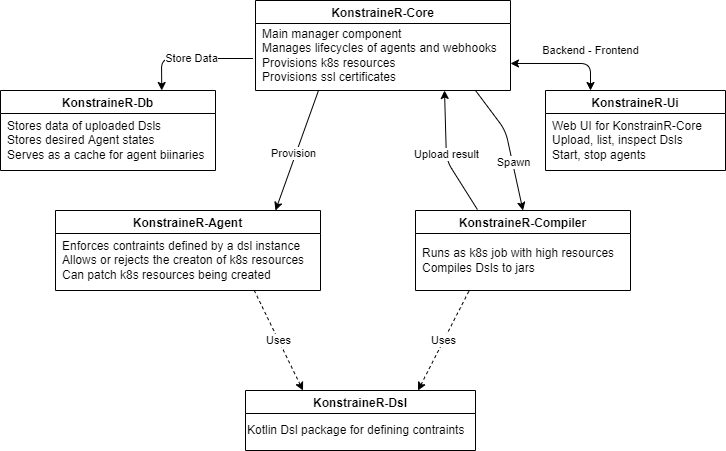
\includegraphics[width=130mm, keepaspectratio]{content_real/25_archPlan/xarch.png}
    \caption{Complex architecture plan}
    \label{fig:comp_arch}
\end{figure}

\subsection{KonstraineR-Core}

The main component in this setup is the KonstraineR-Core. This is an HTTP API server managing the whole application. DSL instances can be uploaded to it, and serves as a store for the uploaded and compiled DSL instances. It handles all tasks related to spawning, starting, configuring, and destroying agents. Most importantly it manages the TLS certificates and webhooks, which are crucial parts of the agent lifecycle management.

\subsubsection{Agent lifecycle}

In Kubernetes, webhooks need to communicate with the Kubernetes API on a secured connection. To achieve this, KonstraineR-Agent instances require a TLS certificate, and need to serve request using the HTTPS protocol. This certificate can be self signed, but in the webhook creation request the CA Key of the certificate must be sent to the Kubernetes API for signing. After this, the Kubernetes API will trust the certificate of the webhook.

The mutating or validation webhooks have their own Kubernetes resource. It is either a \emph{MutatingWebhookConfiguration} or a \emph{ValidatingWebhookConfiguration}. These need to be created in the cluster, so Kubernetes can send the object creation requests to the Pod implementing the webhook.

After the webhook is configured and created in Kubernetes, the Agent can be spawned. Agents are spawned as \emph{deployment}s and they also require a \emph{service}. There are two complicated tasks with the creation of the deployment. First the a TLS certificate must be mounted to the Agent container. Second, the compiled DSL must be also mounted to the container. At this point I haven't decided what is the best way to achieve this. Automated Agent spawning is not the scope of this semester. For now, I styed with copying the required files to the Agent container by hand.

When an Agent is deleted there is a cleanup job to do. All the created Kubernetes resources associated with the given Agent must be deleted alongside with the \emph{WebhookConfiguration}. The deletion of the \emph{deployment}, \emph{service} and \emph{WebhookConfiguration} must be atomic.

\subsubsection{DSL store}

Rules, constraints defined using the KonstraineR-Dsl can be uploaded to the Core component. To apply a ruleset, first it must be uploaded. The compilation of the rule will start right after the upload.

It is simply a HTTP API with support for the CRUD operations. DSLs can be uploaded, listed, inspected, updated and deleted.

\subsection{KonstraineR-Db}

This is an SQL database, providing persistence for the KonstraineR-Core. It stores all the uploaded DSL instances, their statuses and the serves as a cache for the compiled DSLs.

The status of the DSL instance represents the compilation state of the instance, whether it is being compiled, successfully compiled, or outdated and needs to be recompiled.

Caching the compiled DSL instances is very important. A DSL instances are compiled to JVM byte code using gradle, so it can take a long to compile an instance. Compiling a DSL before each launch of an agent would significantly increase the startup time of the agent. A long startup time would mean a relatively long outage when the pod of an already existing agent gets destroyed. This could happen for many reasons, such as the pod gets evicted, deleted manually by an administrator or just simply encounters a fatal error.


\setlength{\parindent}{0pt}
\setlength{\parskip}{0.6em}

%----------------------------------------------------------------------------
\chapter{Methods for enforcing constraints}
\label{sec:enforcingMethods}
%----------------------------------------------------------------------------

There are two major ways of enforcing constraints. The first method is based on the inspection of the current state, the second method is based on capturing events and validating them. For example we can reject an event if the change created by that event would violate some requirements.

\section[State inspection based]{Enforcing constraints based on the inspection of current state}

By inspecting the current state, we can create a report of the requirement violations, and admins can fix the violations with the help of the report. On the other hand we can try to automatically fix those violations.

Both methods have advantages and disadvantages. Fixing the violations automatically is much faster and cheaper. There is no need to spend the precious hours of engineers on refactoring tasks, however this is like sweeping the problem under the rug. 

The incorrect version will remain in version control and the problem will be hidden from the engineers. Furthermore it can cause instability, outages and longer update times. When deploying a new version of the application, the fixed version will be overwritten with the new one, because the fix was never pushed to version control. Of course the new version will be automatically patched, but that will take time and this will also hide the true result of the update, because the update does not finish when the `helm upgrade' executes and the deployment becomes healthy, but when the automatic patch finishes. What would happen in the case of a failed automatic patch? The CI/CD pipeline that triggered the update has already finished with success, so an automatic rollback by the CI/CD pipeline is not possible in this case.

Fixing most of these problems is possible, however very complex and requires making the patching semi automatic with manual validation of the patch. If the manual validation is required, it is better to fix the problem manually and push it to version control to make it permanent.





\section[Event validation based]{Enforcing constraints based on event validation}

Once the state of the cluster is diagnosed, tickets can be created for admins to fix them. However when new components are introduced to the cluster, those components can violate some non-functional requirements, therefore making more work for admins.


We can deny events that would create violations, or we can patch them. Patches should be used with caution. Some time 



Event validation can also be used to other purposes. Delete denied.

webhooks generaly anything sidecar injection, 




\section{Domain specific language}
\label{sec:dsl}

This section explains how I created the Konstrainer DSL. I won't explain the details of creating each keyword, as many of them belong to specific categories and share similar patterns within the same category.

\subsection{Basic concepts}

My DSL has three mayor concepts: blocks, properties, and setter functions. The code snippet \ref{code:lang1} explains what they are and provides an example for each.

\begin{minipage}{\linewidth}
\begin{lstlisting}[caption={Language concepts},language=Kotlin,label=code:lang1]
// The car keyword opens a new block
car { 
  // The block of the car keyword starts here
  color = "red" // This is a property
  color("red") // This is a setter function
  // The block of the car keyword ends here
}
\end{lstlisting}
\end{minipage}

Properties and setter functions usually can only be used within the context of a block. This is how it makes sense in the language, for example you can set the color of the car, but it does not make sense to set the color of the top level world. Additionally, the implementation of a block also restricts where other keywords can be used.

\subsection{Blocks}
 
The \ref{code:lang1} example can be implemented similarly like in the \ref{code:lang2} code snippet.

Most blocks follow the same pattern. There is builder function: `car' in this case, whose last argument is an extension method on a builder class, in this case the `CarBuilder.' Newly accessible keywords in the `car' block are all member functions or properties of the builder class. Lastly, there is a model class, specifically the `CarModel' which holds all the necessary data for a car in this case. The builder function always has an internal build function, making it inaccessible to the DSL user, and it returns an instance of the model class.

\begin{minipage}{\linewidth}
\begin{lstlisting}[caption={Basic idea behind a block},language=Kotlin,label=code:lang2]
class CarModel(val color: String)
class CarBuilder {
  var color: String ...
  fun color(value: String) ...
  internal fun build(): CarModel ...
}
fun car(setup: CarBuilder.() -> Unit): CarModel {
  ...
}
\end{lstlisting}
\end{minipage}

There are two kinds of blocks. The first kind simply describes a configuration or calculates a value, like the `namespaceSelector' or `webhookConfigBundle'. The other describes a complex behavior, which can only be evaluated at certain events, for example the `report', `kubectl' and `behavior' blocks. I refer to the first group as `startup-time' evaluated blocks because a model object can be built without an input. This typically occurs when the agent running the script starts up. I call the second group as `runtime-evaluated blocks' because an input is required to evaluate them, such as a webhook request, or a Kubernetes client.

The pattern I'm using for the startup-time block has a name, it is the Type-safe builders~\cite{TypeSafeBuilders} pattern. The \ref{code:lang3} code snippet highlights the most important elements of the pattern.

\begin{minipage}{\linewidth}
\begin{lstlisting}[caption={Type-safe builders example},language=Kotlin,label=code:lang3]
typealias CarBuilderFunction = CarBuilder.() -> Unit
class CarModel(...)
class CarBuilder {
  ...
  internal fun build(): CarModel {
    // Validations
    ...
    return CarModel(...)
  }
}
fun car(setup: CarBuilderFunction): CarModel {
  val builder = CarBuilder()
  builder.setup()
  return builder.build()
}
// This is tha same, but shorter
fun car(setup: CarBuilderFunction) = CarBuilder().apply(setup).build()
\end{lstlisting}
\end{minipage}

Runtime-evaluated blocks are created differently. Their builder functions don't call the `build' function of the builder class, because the input required to create the model does not exist yet. I will use the `report' block to explain how they are implemented.

\begin{minipage}{\linewidth}
\begin{lstlisting}[caption={Builder function of the report block},language=Kotlin,label=code:runtimeblock0]
class ServerModel(..., val _report: ReportProviderFunction?)
class ServerBuilder {
  private val _report: ReportProviderFunction? by setMaxOnce()
  fun report(behavior: ReportProviderFunction) {
    _report = behavior
  }
  internal fun build() = Server(..., _report)
}
\end{lstlisting}
\end{minipage}

The \ref{code:runtimeblock0} snippet shows how the builder function of a runtime block, specifically the `report' block looks like. The `build' function is not called here; instead, the behavior lambda is stored in a variable of the parent block. The invocation of the `build' function is moved to the code of the agent. This isn't how it is actually implemented, but the \ref{code:runtimeblock1} gives the basic idea of how it could be implemented. Here, the input data is a Kubernetes client, and it is passed to the constructor of the builder class.

\begin{minipage}{\linewidth}
\begin{lstlisting}[caption={Build a report},language=Kotlin,label=code:runtimeblock1]
fun generateReport(
    k8s: KubernetesClient, 
    provider: ReportProviderFunction
  ): Report {
  val builder = ReportBuilder(k8s)
  builder.provider()
  return builder.build()
}
\end{lstlisting}
\end{minipage}

The \ref{code:runtimeblock2} snippet show the implementation of the builder class and the provider.

\begin{minipage}{\linewidth}
\begin{lstlisting}[caption={Report builder class and provider},language=Kotlin,label=code:runtimeblock2]
typealias ReportProviderFunction = ReportBuilder.() -> Unit
class ReportBuilder(private val k8s: KubernetesClient) {
  // All the child keywords of the report block
  ...
  fun build(): Report { ... }
}
\end{lstlisting}
\end{minipage}

The actual implementations of the runtime-evaluated blocks vary in the codebase due to the evolution of the DSL. Still, this section explains the core idea. It could be a potential future improvement to streamline the implementation of each block.

\subsection{`setExactlyOnce' and `setMaxOnce'}

All properties can only be set once, or in the case of setter functions, invoked once. This is to avoid inadvertent overwrites and to enhance script readability. The enforcement of this language constraint is carried out through the `setExactlyOnce' and 7setMaxOnce' property delegates. Kotlin has unique a feature called property delegates, which enables to define a custom behavior to a set of properties. This custom behavior can be added to a library, eliminating the need to copy and paste the behavior into every getter and setter. Instead, you simply utilize the delegate. For detailed information, read the official Kotlin documentation on the topic: \url{https://kotlinlang.org/docs/delegated-properties.html}. Here, I will just show a small example and explain how my custom property delegates work.

\begin{minipage}{\linewidth}
\begin{lstlisting}[caption={Lazy getter in Java},language=Java,label=code:lazy0]
class A {
  private String foo;
  public getFoo() {
    if (foo == null) 
      foo = calculateFoo(); // This is a resource intese operation
    return foo;
  }
}
\end{lstlisting}    
\end{minipage}

\begin{minipage}{\linewidth}
\begin{lstlisting}[caption={Lazy property in Kotlin},language=Kotlin,label=code:lazy1]
class A {
  val foo by lazy(::calculateFoo)
}
\end{lstlisting}
\end{minipage}

The \ref{code:lazy0} and \ref{code:lazy1} code snippets illustrates how the lazy\footnote{\url{https://en.wikipedia.org/wiki/Lazy_initialization}} behavior can be implemented in Java and in Kotlin. The lazy behavior involves delaying the calculation of a value until it is read, after which it is cached. The Java code snippet shows the issue. When implementing custom behavior for a getter, it must be written each time for every getter with the same behavior. In Kotlin, this behavior can be delegated, making the code not only less bloated but also less prone to copy and paste errors.

\begin{lstlisting}[caption={setExactlyOnce implementation},language=Kotlin,label=code:setonce]
class setExactlyOnce<T : Any>() : ReadWriteProperty<Any, T> {
  constructor(default: T?) : this() {
    _value = default
  }
  private var _alreadySet = false
  private var _value: T? = null

  override fun getValue(thisRef: Any, property: KProperty<*>): T {
    return _value ?: throw FieldNotSetException(
      "Property ${property.name} not set."
    )
  }
  override fun setValue(thisRef: Any, property: KProperty<*>, value: T) {
    if (_alreadySet)
      throw MultipleSetException(
        "Property ${property.name} can only be set once."
      )
    _alreadySet = true
    _value = value;
  }
}

// Usage:
// A clusterRole can assigned to an agend maximum once
var clusterRole by setMaxOnce<ClusterRoleName>()
// behavior of webhook can only be set exactly once,
// and has no default value
private var behavior: WebhookBehaviorProvider by setExactlyOnce()
// operations of a webhook can only be set exactly once,
// and has a default value
private var _operations: Array<out String>
    by setExactlyOnce(defaults.operations)
\end{lstlisting}

The \ref{code:setonce} code snippet demonstrates how the `setExactlyOnce' property delegate is implemented. To fully understand why this seemingly complicated syntax was needed, read the official documentation which explains it in detail. What's important here is, that there is an optional default value which can be set when creating a property. The default value is stored in a private backing field: `\_value', which is null, in case there is no default value. 

When the value is set, the delegate checks the `\_alreadySet' flag. If it is true, an exception is raised; otherwise, it sets the value and the flag. The inclusion of the flag is necessary because a simple null check cannot differentiate between an already set value and a default value.

When the value is read, the delegated checks if the `\_value' is null. If it is, then it raises an exception. However, in the case of the `setMaxOnce' delegate, this check does not exist.

I will not show the implementation of `setMaxOnce' because it closely resembles `setExactlyOnce'.

Error messages are not currently aggregated into a centralized view; instead, they can be found in the logs of either the core component or the agent. A potential future improvement could involve collecting and displaying these error messages as build-time errors.

\subsection{JSON utilities}

The language has unique keywords for JSON parsing. They do not fall into the main categories of blocks and properties, but they are unique. They look more like continuous natural English language. Their implementation is a bit complicated and to understand it, you must first understand some basic concepts of Kotlin.

In Kotlin there are infix functions. You can add the `infix' modifier to an extension function to make it callable using the infix notation. See the \ref{code:infix} code snippet for an example or read the official documentation for more details: \url{https://kotlinlang.org/docs/functions.html#infix-notation}

\begin{minipage}{\linewidth}
\begin{lstlisting}[caption={Infix functions},language=Kotlin,label=code:infix]
infix fun Int.plus(that: Int): Int {
  return this + that
}
// Invocation:
val x = 5 plus 6  // Infix notation
val y = 5.plus(6) // This does the same as above
\end{lstlisting}
\end{minipage}

The second concept you must understand is treating objects as tokens. Objects can be utilized in various ways, but what's important for this section is their ability to create special tokens. You can define two functions with the same name but different arguments. If these arguments are of this kind of tokens, they can be used for pattern matching as shown in the \ref{code:patternobj} code snippet.

\begin{minipage}{\linewidth}
\begin{lstlisting}[caption={Pattern matching},language=Kotlin,label=code:patternobj]
object Token1
object Token2

fun foo(o: Token1) {
  ...
}
fun foo(o: Token2) {
  ...
}
// Invocation
val x = Token2
foo(x)      // Runs the second foo function
foo(Token1) // Runs the first foo function
\end{lstlisting}
\end{minipage}

Combining these Kotlin language features can be used to create fluent, natural language-like constructs. The \ref{code:parseAs} code snippet demonstrates how these language concepts are employed to implement the JSON parsing aspects of the Konstrainer DSL.

\begin{minipage}{\linewidth}
\begin{lstlisting}[caption={JSON parsing implementation},language=Kotlin,label=code:parseAs]
infix fun JsonElement.jqx(selector: String): JsonElement {
  ...
}

object int
object bool
object double
object string

infix fun JsonElement.parseAs(type: int): Int? = 
  nullGuard { /* Function defining how to get JSON field as Int*/ }
infix fun JsonElement.parseAs(type: bool): Boolean? = nullGuard { ... }
infix fun JsonElement.parseAs(type: double): Double? = nullGuard { ... }
infix fun JsonElement.parseAs(type: string): String? = nullGuard { ... }

// Usage:
val x = jsonElement jqx "/foo/bar" parseAs string
\end{lstlisting}
\end{minipage}

`jqx' is an infix function with a return type of JsonElement. `parseAs' is also an infix function with the type JsonElement as a receiver, so `jqx' and `parseAs' commands can be chained. There is a token created for every the primitive types that can occur in a JSON, and there is a corresponding `parseAs' function for each token. This setup facilitates the extraction of all types from a JSON structure. The `nullGuard' is a private function that return null if the conversion can not happen, for instance, due to a type mismatch or non-existing JSON field. Otherwise, it returns the converted value. The conversion function is defined in its block.

\chapter{Case study 2: Creating new constraints}
\label{chap:case_study2}

The \ref{chap:case_study1} chapter only showed the capabilities of the Konstrainer framework, but did not show how to write a more advanced script, because the \nameref{chap:konst_dsl} chapter was a prerequisite for that. This chapter will continue the case study.

\section{Writing your own policies}

Let's assume the company has introduced some custom policies and, now they want to enforce them using Konstrainer. Start with a very simple policy: All images must come from the internal company registry.

To enforce this, first let's detect which pods violate this policy:

Create a file with the company-policies.kt file with the following content:

\begin{lstlisting}[caption={Report skeleton},language=Kotlin,label=code:todo]
package me.btieger

import me.btieger.dsl.*

const val companyPrefix = "tiegris/"
val companPolicies = server("company-policies") {
  report {

  }
}
\end{lstlisting}

This script has an empty report so far. As described in the \ref{sec:report} section, we should fetch the list of pods and create an aggregation group. In this case, no additional processing is needed.

\begin{lstlisting}[caption={Aggregation group},language=Kotlin,label=code:todo]
report {
  val pods = kubelist { pods() }
  aggregation("Pods", pods) {

  }
}
\end{lstlisting}

To decide if all the containers of a pod are using images only from the company registry, we must specify this requirement with mathematical precision, using first order logic. Here are two continuous sentences which, express the requirement with first order logic.

`Tag the pod, if any of its containers image does not start with the company prefix.'

`Do not tag the pod, if all of its containers image starts with the company prefix.'

\begin{lstlisting}[caption={Tag pods},language=Kotlin,label=code:todo]
report {
  aggregation("Pods", kubelist { pods() }) {
    tag("Image not from company registry") {
      item.spec.containers.any { !it.image.startsWith(companyPrefix) }
    }
  }
}
\end{lstlisting}

The script accesses the Kubernetes API, but to do that successfully, it needs authorization. We need to associate a \emph{ClusterRole} to the agent. In the demo files there is also a \emph{ClusterRole} definition. We want our agent to be least privileged, so we are only giving it read access to the pods.

\begin{lstlisting}[caption={TODO},language=Kotlin,label=code:todo]
package me.btieger
import me.btieger.dsl.*

const val companyPrefix = "tiegris/"
val companyPolicies = server("company-policies") {
  clusterRole = "read-pods"
  report {
    aggregation("Pods", kubelist { pods() }) {
      tag("Image not from company registry") {
        item.spec.containers.any { !it.image.startsWith(companyPrefix) }
      }
    }
  }
}
\end{lstlisting}

The line: `clusterRole = ReadAny` assigns the ReadAny clusterrole to the agent by creating a clusterrolebinding during the deployment of the agent. The ReadAny clusterrole is created with the Konstrainer installation, it gives read access to all resources in the cluster.

Let's test the script now. If we upload, and deploy the script, we should see it working:

\begin{figure}[h]
  \centering
  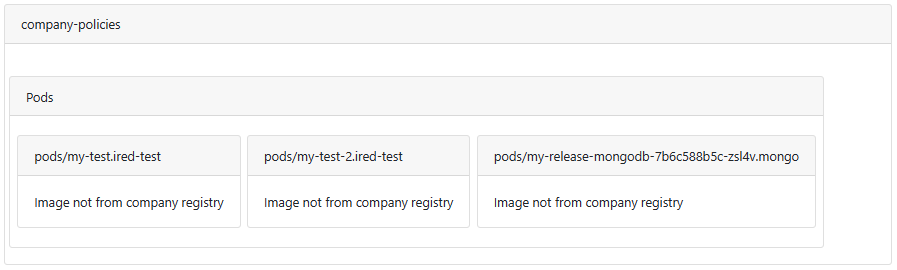
\includegraphics[width=130mm, keepaspectratio]{content/60_caseStudy2/company_policies_1.png}
  \caption{Report generated by the script}
  \label{fig:report}
\end{figure}

The report shows that there are 3 pods, which use images outside from the company registry.

Now lets do the enforcing part. Put this code inside the server block.

\begin{lstlisting}[caption={TODO},language=Kotlin,label=code:todo]
webhook("only-internal-registry") {
  operations(CREATE, UPDATE)
  apiGroups(APPS)
  apiVersions(ANY)
  resources(DEPLOYMENTS, STATEFULSETS, DAEMONSETS)
  namespaceSelector { }
  failurePolicy(FAIL)
  behavior {
    allowed {
      podSpec!!.containers.all { it.image.startsWith(companyPrefix) }
    }
    status {
      message = "All images must be from the company registry."
    }
  }
}
\end{lstlisting}

To create a rule, we need to add a `webhook` block. It needs a unique name. Lets name it "only-internal-registry". We need to define which events should the webhook listen to. In this example the webhook listens to the creation or update of any deployments, statefulsets and daemonsets.

The more interesting part is the behavior block. It describes how should the webhook behave when a request arrives. Inside the behavior block we can access the request body using many ways. One of them is the podSpec keyword. It is a shortcut to the `.spec.template.spec` of a deployment, statefulset or daemonset.

In the allowed block we can specify when to allow or reject an event. In this case we only accept events when the all the containers of the pod has an image starting with the the company prefix.

In the status block we define the error message in case the event is rejected.

Lets deploy and test our newly created agent dsl. On the monitors view we can see that the pods inside the ired-test namespace use images outside of the company registry, and the mongodb also uses an image from docker.io instead of the company registry.

We can also test that we can no longer create resources which use images outside from the company registry:

\begin{lstlisting}[caption={TODO},language=bash,label=code:bashx]
kubectl create ns policy-test
kubectl apply -f k8s/test-policy.yaml -n policy-test
\end{lstlisting}

We should get this error:

\begin{lstlisting}[caption={TODO},language=bash,label=code:todo]
Error from server: error when creating "k8s/test-policy.yaml": admission webhook "only-internal-registry.btieger.me" denied the request: All images must be from the company registry.
\end{lstlisting}

\begin{lstlisting}[caption={TODO},language=bash,label=code:bashx]
yq eval 'select(.kind == "Deployment").spec.template.spec.containers[0].image = "tiegris/apples-users"' k8s/test-policy.yaml -i
kubectl apply -f k8s/test-policy.yaml -n policy-test
\end{lstlisting}

This error shows that our rule works and is enforced.

This is the end of the demo. In this demo we saw the basic capabilities of the Konstrainer platform, some use-cases, and how to create our own rules.


% Ktor web keretrendszer: lábbal hajtós, kényelmes könnyű dinamikus koncig, kiforratlan, nincsenek best practice-ek -> konklúzió

% security

% esettanulmány: 

% dsl általánosan, ami készült <- esettanulmányon keresztül, előtte

% 

%~~~~~~~~~~~~~~~~~~~~~~~~~~~~~~~~~~~~~~~~~~~~~~~~~~~~~~~~~~~~~~~~~~~~~~~~~~~~~~~~~~~~~~


% Acknowledgements
%~~~~~~~~~~~~~~~~~~~~~~~~~~~~~~~~~~~~~~~~~~~~~~~~~~~~~~~~~~~~~~~~~~~~~~~~~~~~~~~~~~~~~~
% %----------------------------------------------------------------------------
\chapter*{\koszonetnyilvanitas}\addcontentsline{toc}{chapter}{\koszonetnyilvanitas}
%----------------------------------------------------------------------------

Szeretnék köszönetet mondani a konzulensemnek, Elekes Mártonnak az áldozatos munkájáért és segítőkészségért. Továbbá köszönöm Dr. Micskei Zoltánnak, hogy bevezette számomra SysML v2 nyelv alapjait.



% List of Figures, Tables
%~~~~~~~~~~~~~~~~~~~~~~~~~~~~~~~~~~~~~~~~~~~~~~~~~~~~~~~~~~~~~~~~~~~~~~~~~~~~~~~~~~~~~~
%\listoffigures\addcontentsline{toc}{chapter}{\listfigurename}
%\listoftables\addcontentsline{toc}{chapter}{\listtablename}


% Bibliography
%~~~~~~~~~~~~~~~~~~~~~~~~~~~~~~~~~~~~~~~~~~~~~~~~~~~~~~~~~~~~~~~~~~~~~~~~~~~~~~~~~~~~~~
\addcontentsline{toc}{chapter}{\bibname}
\bibliography{bib/mybib}


% Appendix
%~~~~~~~~~~~~~~~~~~~~~~~~~~~~~~~~~~~~~~~~~~~~~~~~~~~~~~~~~~~~~~~~~~~~~~~~~~~~~~~~~~~~~~
%\include{content/appendices}

%\label{page:last}
\end{document}
